% !TEX root = Sudoku.tex

\begin{figure}[t]
    \begin{center}
        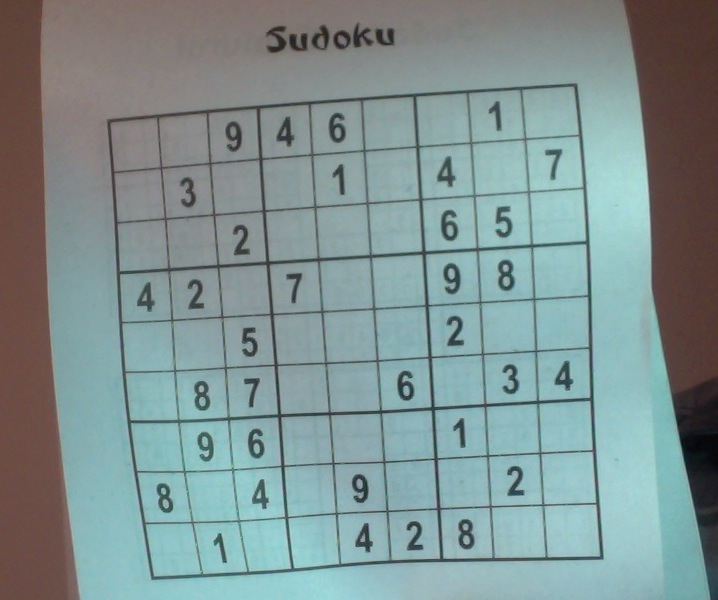
\includegraphics[width=.5\textwidth]{Abbildungen/Input}
    \end{center}
    \caption{Das verwendete Testbild}
    \label{fig:Input}
\end{figure}

\section{Vorgehensweise}
Zum Lösen dieser Aufgabe wird die Programmiersprache \emph{Python 2.7}\footnote{http://www.python.org} verwendet.
Für diese steht in Form der Open-Source Library \emph{OpenCV}\footnote{http://docs.opencv.org} eine leistungsstarke Bibliothek zur Bildverarbeitung zur Verfügung.
OpenCV selbst ist in C++ geschrieben, bietet jedoch entsprechende Python-Bindings an.

Für die Erkennung der Ziffern wird die von Google entwickelte \emph{Tesseract}\footnote{https://code.google.com/p/tesseract-ocr}-Library verwendet. Auch für diese existieren Python-Bindings in Form von \emph{python-tesseract}\footnote{https://code.google.com/p/python-tesseract}.

Als Eingangsbild wird das Bild aus Abbildung~\ref{fig:Input} verwendet. Dieses wurde mit der Webcam eines MacBook Pro aufgenommen.

\subsection{Bild-Vorverarbeitung}
Das Bild wird zunächst in Graufstufen umgesetzt, da Farben vernachlässigt werden können.

Anschließend wird das Bild mit einem adaptiven Threshold binärisiert. Ein einfacher Threshold eignet sich nicht, da die Licht- und Kontrastverhältnisse unbekannt sind.

Um das Rauschen zu entfernen, wird noch ein 3x3 Medianfilter angewendet.

\begin{lstlisting}
def process(frame):
    #
    # 1. preprocessing
    #
    gray = cv2.cvtColor(frame, cv2.COLOR_BGR2GRAY)
    binary = cv2.adaptiveThreshold(
        src=gray, maxValue=255,
        adaptiveMethod=cv2.ADAPTIVE_THRESH_GAUSSIAN_C,
        thresholdType=cv2.THRESH_BINARY, blockSize=11, C=2)
    blurred = cv2.medianBlur(binary, 3)
\end{lstlisting}

\begin{figure}[H]
    \subfigure{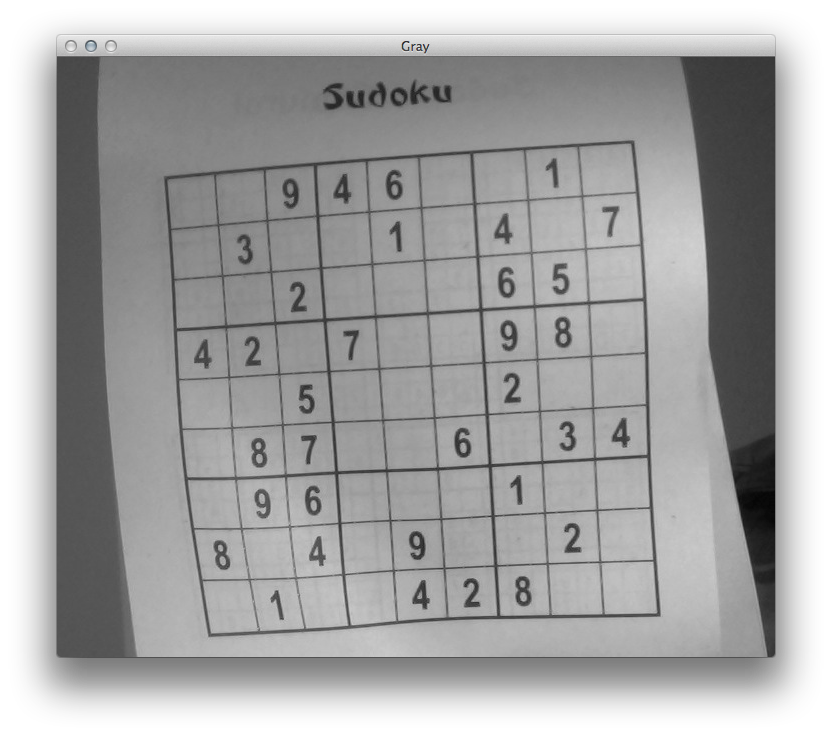
\includegraphics[width=0.49\textwidth]{Abbildungen/gray}}
    \subfigure{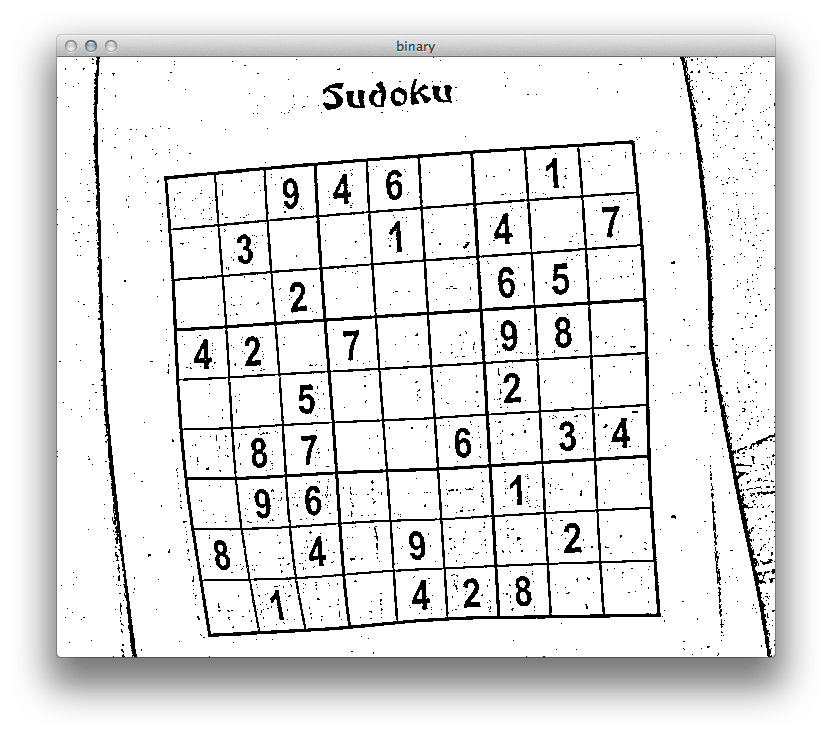
\includegraphics[width=0.49\textwidth]{Abbildungen/binary}}
\end{figure}
%
\begin{figure}[H]
    \centering
    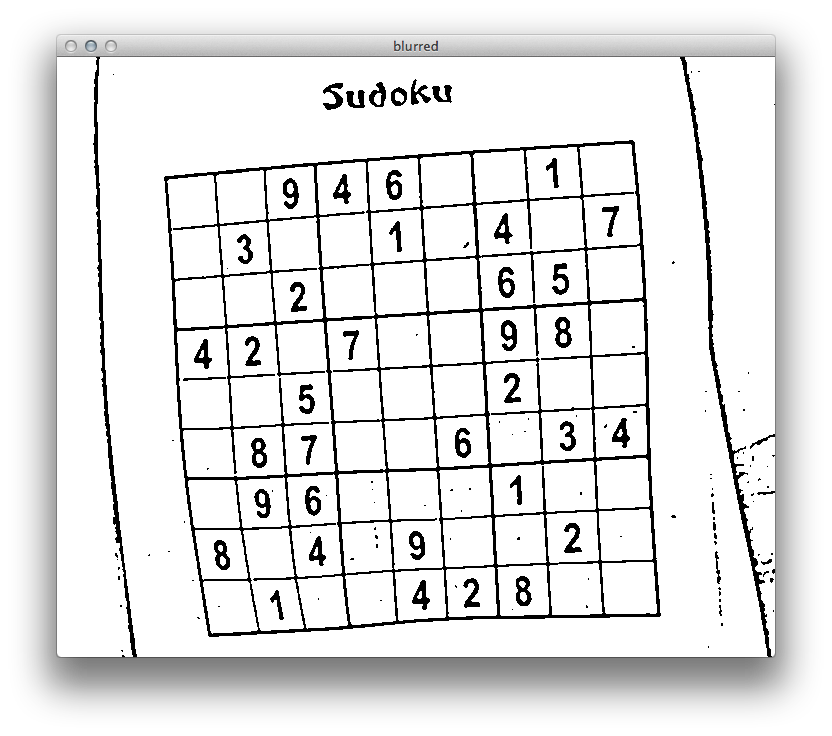
\includegraphics[width=.5\textwidth]{Abbildungen/median}
    \caption{Nach der Bild-Vorverarbeitung (Graufstufen, binärisiert, gefiltert)}
\end{figure}

\subsection{Sudoku lokalisieren}
Um die Position des Sudokus zu bestimmen, werden zunächst alle Konturen im Bild ermittelt.
Dazu muss das binärisierte Bild invertiert werden, da der Algorithmus weiße Pixel als Objektpixel erwartet.
Alle Konturen werden über folgende Kriterien gefiltert:

\begin{enumerate}
    \item Das umschließende Rechteck muss annähernd quadratisch sein. Dazu werden die Seitenverhältnisse überprüft.
    \item Um kleine Konturen auszuschließen, wird eine Mindestfläche vorgegeben.
    \item Hinzu kommt ein Mindestwert für das Verhältnis der Konturfläche zur Fläche des umschließenden Rechtecks, um beispielsweise ``L''-förmige Konturen auszuschließen.
\end{enumerate}

Von allen Konturen, die diese Bedingungen erfüllen, wird diejenige mit der größten Konturfläche ausgewählt.

\begin{lstlisting}
    # try to find the sudoku
    contours, _ = cv2.findContours(image=cv2.bitwise_not(blurred),
                                   mode=cv2.RETR_LIST,
                                   method=cv2.CHAIN_APPROX_SIMPLE)
    sudoku_area = 0
    sudoku_contour = None
    for cnt in contours:
        area = cv2.contourArea(cnt)
        x, y, w, h = cv2.boundingRect(cnt)
        if (0.7 < float(w) / h < 1.3     # aspect ratio
                and area > 150 * 150     # minimal area
                and area > sudoku_area   # biggest area on screen
                and area > .5 * w * h):  # fills bounding rect
            sudoku_area = area
            sudoku_contour = cnt
\end{lstlisting}


\subsection{Sudoku isolieren und transformieren}
Das umschließende Rechteck der Kontur stellt nur in Spezialfällen die tatsächliche Kontur des Sudokus dar.
Um die Eckpunkte des Sudokus im Bild zu ermitteln, wird daher die gefundene Kontur mit dem \emph{Ramer–Douglas–Peucker}\footnote{http://de.wikipedia.org/wiki/Douglas-Peucker-Algorithmus}-Algorithmus durch einem Linienzug approximiert.
Über den Parameter \emph{epsilon} lässt sich der maximal gültige Fehler der Approximation einstellen.
So kann erreicht werden, dass die Approximation aus genau vier Punkten besteht, die dann die Eckpunkte darstellen.

Der zulässige Fehler ist abhängig vom Umfang der Kontur.
Er muss so eingestellt werden, dass leichte Verformungen noch zulässig sind, die Ecken aber zuverlässig erkannt werden.

\begin{lstlisting}
    #
    # 3. separate sudoku from background
    #
    if sudoku_contour is not None:

        # approximate the contour with connected lines
        perimeter = cv2.arcLength(curve=sudoku_contour, closed=True)
        approx = cv2.approxPolyDP(curve=sudoku_contour,
                                  epsilon=0.1 * perimeter,
                                  closed=True)
\end{lstlisting}

Wenn die Kontur mit vier Punkten approximiert werden kann, wird zur Separation eine Maske erstellt.
Dazu wird auf einen schwarzen Hintergrund die Kontur des Sudokus gezeichnet und weiß gefüllt.
Dieses Bild wird invertiert und mit dem bereits binärisierten Bild verodert.
Das Resultat ist das isolierte Sudoku auf weißem Hintergrund.
Dies ist notwendig, da sonst auf schwarzem Hintergrund die äußerste Feldbegrenzung verschwindet.

\begin{lstlisting}
    if len(approx) == 4:
        # successfully approximated
        # we now transform the sudoku to a fixed size 450x450
        # plus 50 pixel border and remove the background

        # create empty mask image
        mask = np.zeros(gray.shape, np.uint8)
        # fill a the sudoku-contour with white
        cv2.drawContours(mask, [sudoku_contour], 0, 255, -1)
        # invert the mask
        mask_inv = cv2.bitwise_not(mask)
        # the blurred picture is already thresholded so this step shows
        # only the black areas in the sudoku
        separated = cv2.bitwise_or(mask_inv, blurred)
\end{lstlisting}

\begin{figure}[H]
    \begin{center}
        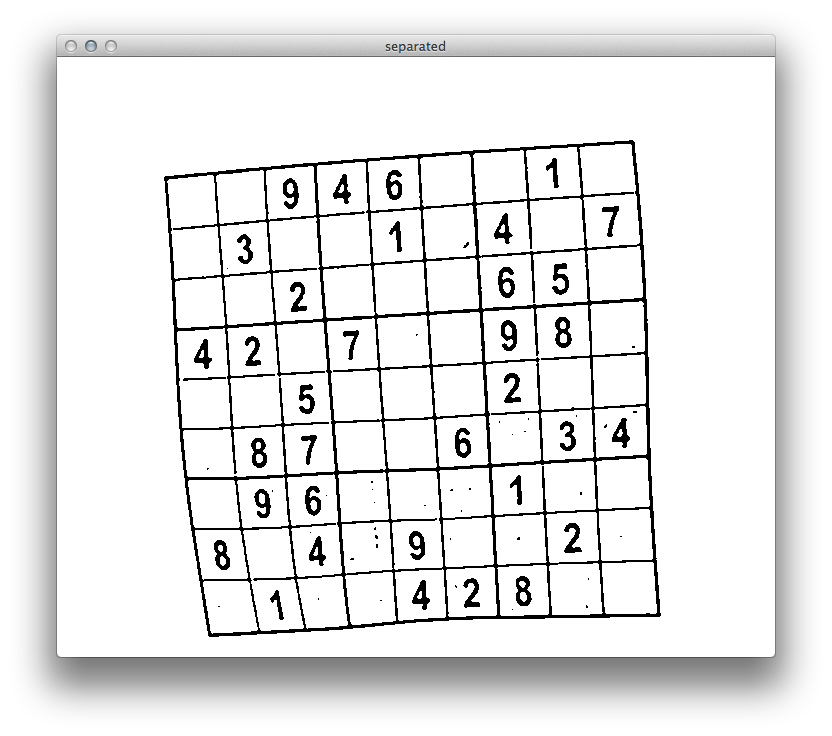
\includegraphics[width=.5\textwidth]{Abbildungen/separated}
    \end{center}
    \caption{Das vom Hintegrund getrennte Sudoku.}
\end{figure}

Das isolierte Sudoku wird anhand der approximierten Eckpunkte perspektivisch zu einem Quadrat der Größe 450x450px transformiert.
Je nach Biegung des Papiers sind im Quadrat und an den Außenrändern noch perspektivische Verzerrungen vorhanden. Um zu verhindern, dass diese verzerrten Randbereiche abgeschnitten werden, wird ein zusätzlicher Abstand von 50px hinzugefügt.

Zuerst werden die Eckpunkte des Zielquadrats festgelegt und den approximierten Eckpunkten zugewiesen. Daraus ergibt sich die Transformationsmatrix, die anschließend auf das isolierte Sudoku angewendet wird.

\begin{lstlisting}
    # create a perspective transformation matrix. "square" defines the
    # target dimensions (450x450). The image we warp "separated" in
    # has bigger dimensions than that (550x550) to assure that no
    # pixels are cut off accidentially on twisted images
    square = np.float32([[50, 50], [500, 50], [50, 500], [500, 500]])
    approx = np.float32([i[0] for i in approx])  # api needs conversion
    # sort the approx points to match the points defined in square
    approx = sort_rectangle_contour(approx)

    m = cv2.getPerspectiveTransform(approx, square)
    transformed = cv2.warpPerspective(separated, m, (550, 550))
\end{lstlisting}

\begin{figure}[H]
    \begin{center}
        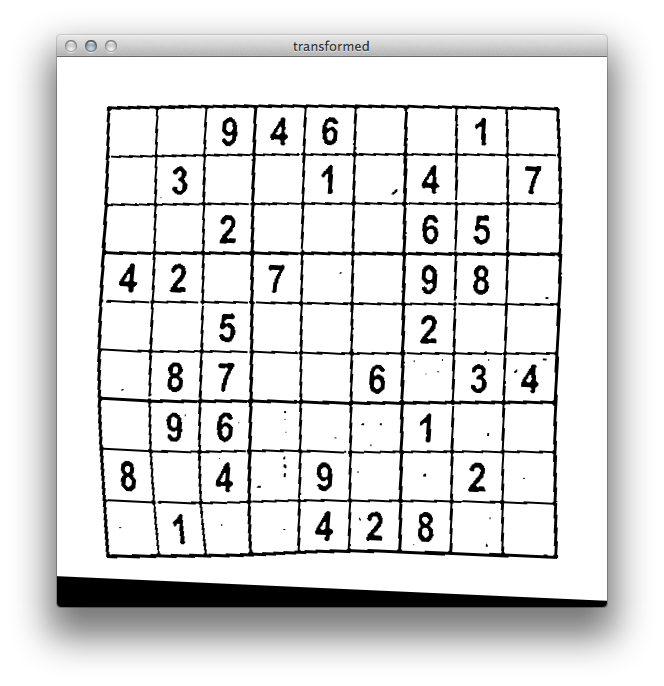
\includegraphics[width=.5\textwidth]{Abbildungen/transformed}
    \end{center}
    \caption{Das perspektivisch auf die richtige Größe transformierte Sudoku.}
\end{figure}


\subsection{Gitteranalyse}
Da die Positionen der Ziffern aufgrund der Wölbung des Papiers nicht fix angenommen werden können, müssen zunächst die Eckpunkte der Einzelzellen gefunden werden.
Dazu werden die Kreuzungspunkte der Gitterlinien bestimmt.

\subsubsection{Linienerkennung}
Zur Erkennung der Kanten wird der Sobel-Operator in X- und Y-Richtung eingesetzt.

\begin{figure}[H]
    \subfigure{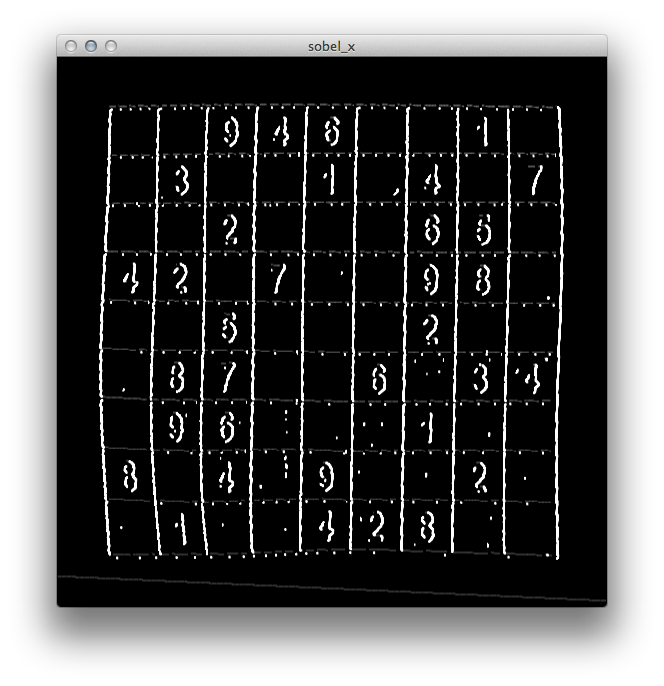
\includegraphics[width=0.49\textwidth]{Abbildungen/sobel_x}}
    \subfigure{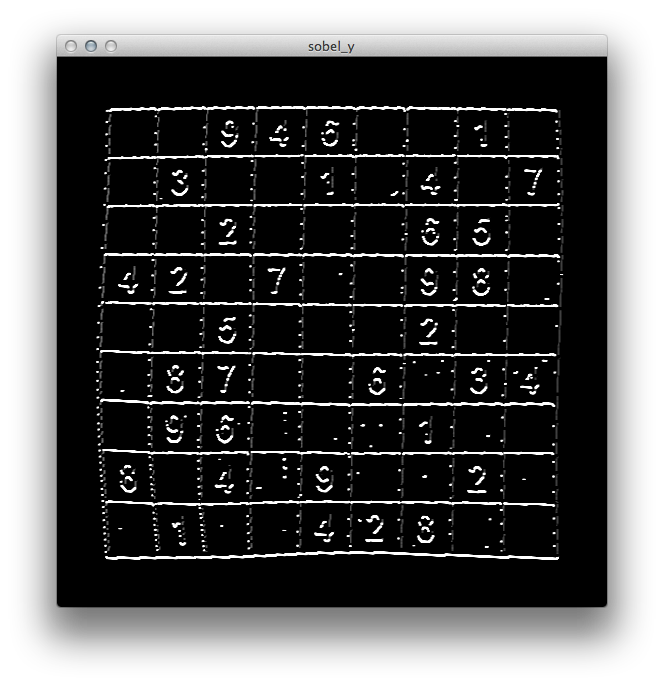
\includegraphics[width=0.49\textwidth]{Abbildungen/sobel_y}}\hfill
    \caption{Erkannte Kanten nach der Sobel-Operation}
\end{figure}

Der Sobel-Operator generiert an den Kreuzungspunkten Fehlstellen, daher sind die Gitterlinien nicht durchgängig und müssen geschlossen werden.
Sie werden durch einen Closing-Operator geschlossen.
Dazu wird das Bild mit dem gleichen Element dilatiert und anschließend erodiert.

Der Sobel-Operator erzeugt Grauwerte im Bild, die durch eine erneute Binärisierung wieder verworfen werden.

\begin{lstlisting}
    # sobel x-axis
    sobel_x = cv2.Sobel(transformed, ddepth=-1, dx=1, dy=0)

    # closing x-axis
    kernel_x = np.array([[1]] * 20, dtype='uint8')  # vertical kernel
    dilated_x = cv2.dilate(sobel_x, kernel_x)
    closed_x = cv2.erode(dilated_x, kernel_x)
    _, threshed_x = cv2.threshold(closed_x, thresh=250, maxval=255,
                                  type=cv2.THRESH_BINARY)
\end{lstlisting}

\begin{figure}[H]
    \subfigure{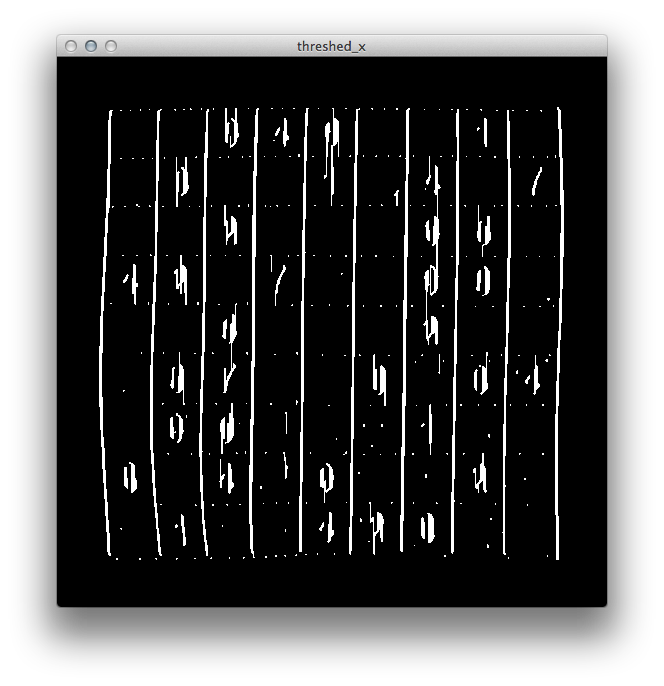
\includegraphics[width=0.49\textwidth]{Abbildungen/threshed_x}}
    \subfigure{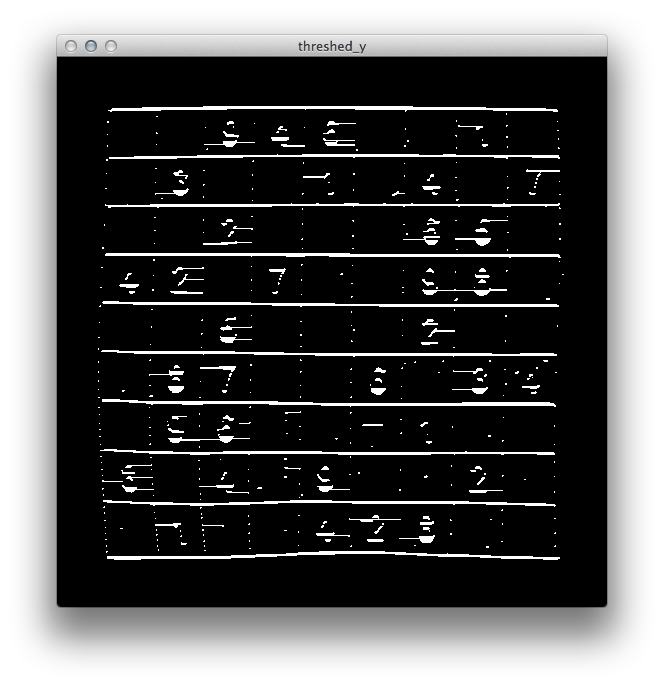
\includegraphics[width=0.49\textwidth]{Abbildungen/threshed_y}}
    \hfill
    \caption{Geschlossene und binärisierte Gitterlinien}
\end{figure}

Aus diesem Bild werden die zehn größten Konturen ermittelt und isoliert, indem die Konturen der Linien auf ein leeres Bild gezeichnet werden.

\begin{lstlisting}
    # generate mask for x
    contours, _ = cv2.findContours(threshed_x, cv2.RETR_TREE,
                                   cv2.CHAIN_APPROX_SIMPLE)
    # sort contours by height
    sorted_contours = sorted(contours, cmp=cmp_height)

    # fill biggest 10 contours on mask (white)
    mask_x = np.zeros(transformed.shape, np.uint8)
    for c in sorted_contours[:10]:
        cv2.drawContours(mask_x, [c], 0, 255, -1)
\end{lstlisting}

\begin{figure}[H]
    \subfigure[vertikal]{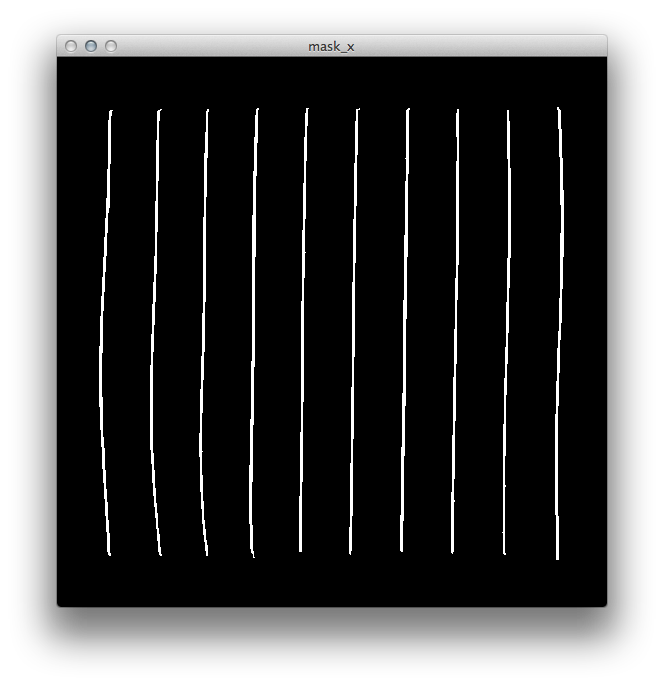
\includegraphics[width=0.49\textwidth]{Abbildungen/mask_x}}
    \subfigure[horizontal]{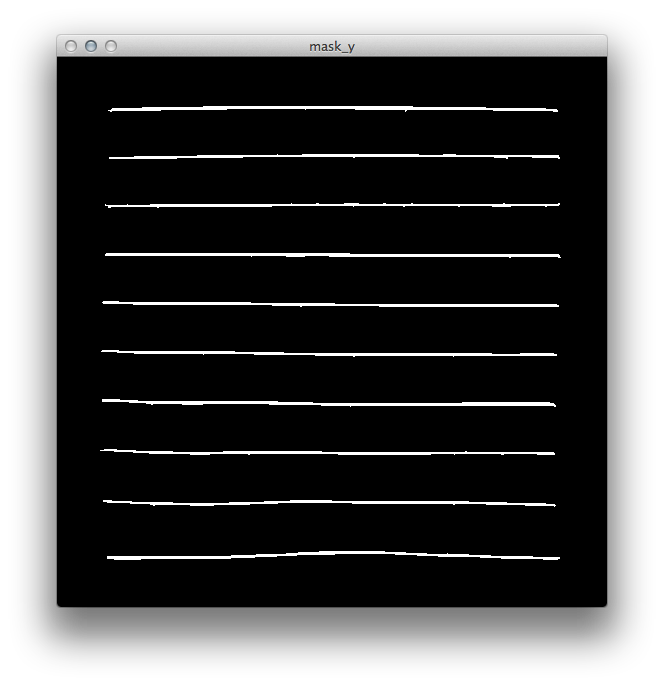
\includegraphics[width=0.49\textwidth]{Abbildungen/mask_y}}
    \hfill
    \caption{Die vereinzelten Linien}
\end{figure}

Die Linien werden durch Dilatation verlängert, damit sichergestellt ist, dass auch an den Randpunkten Überschneidungen entstehen.
Durch Verodern erhält man das vollständige Sudoku-Gitter, durch Verunden nur die Kreuzungspunkte.

\begin{lstlisting}
    dilated_ver = cv2.dilate(mask_x, kernel_x)
    dilated_hor = cv2.dilate(mask_y, kernel_y)
    # now we have the single crossing points as well as the complete grid
    grid = cv2.bitwise_or(dilated_hor, dilated_ver)
    crossing = cv2.bitwise_and(dilated_hor, dilated_ver)
\end{lstlisting}

\begin{figure}[H]
    \subfigure[Kreuzungspunkte (nach Verundung)]{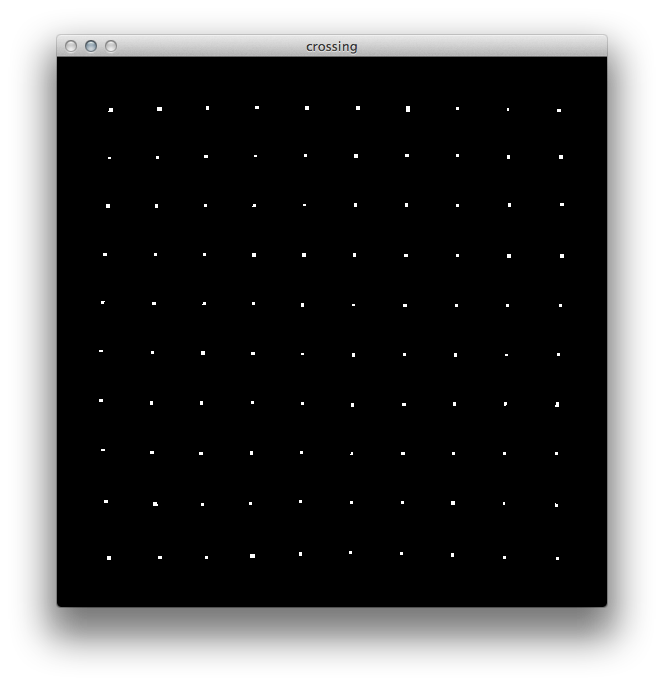
\includegraphics[width=0.49\textwidth]{Abbildungen/crossing}}
    \subfigure[Gitter (nach Veroderung)]{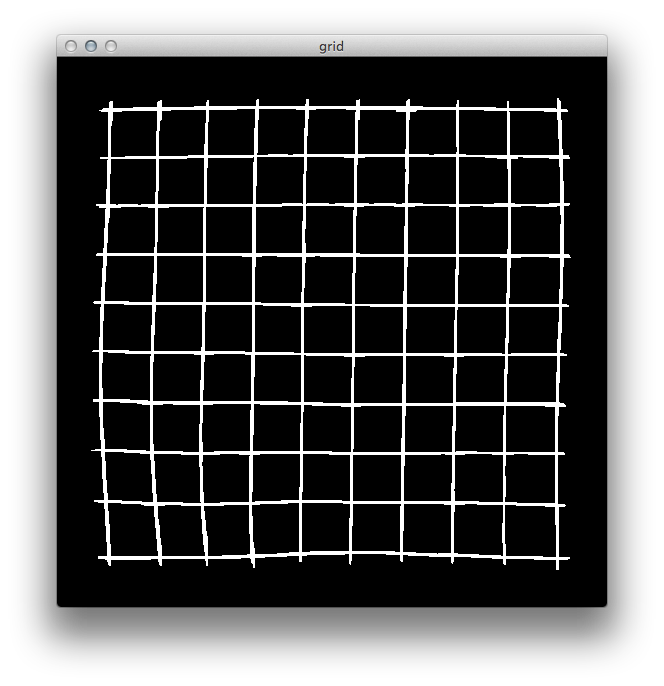
\includegraphics[width=0.49\textwidth]{Abbildungen/grid}}\hfill
    \caption{Erkannte Kreuzungspunkte und Gesamtgitter}
\end{figure}


\subsubsection{Reihenfolge der Kreuzungspunkte}
Wendet man auf das Bild der Kreuzungspunkte eine Konturerkennung an, liegen die erkannten Konturen nicht in einer definierten Reihenfolge vor und müssen daher sortiert werden.

Als Koordinaten der Kreuzungspunkte werden die Mittelpunkte der umschließenden Rechtecke verwendet.
Darauf liegen die Koordinaten in Form einer eindimensionalen Liste vor.

Um diese nach ihrer Position im Bild zu sortieren, müssen die Koordinaten zunächst nach ihrer Y-Position sortiert werden.
Anschließend werden die Koordinaten zu Gruppen zusammengefasst.
Die Gruppengröße entspricht dabei der Anzahl der Koordinaten auf einer Kante des Quadrats, also der Wurzel aus der Anzahl der verfügbaren Punkte.
Innerhalb der Gruppen werden die Koordinaten nun nach ihrer X-Position sortiert und die Gruppen anschließend wieder aufgelöst.

Die Funktionen hierfür kommen aus der Python-Library \emph{numpy}\footnote{http://www.numpy.org}, welche speziell für Matrixoperationen konzipiert wurde.

\begin{lstlisting}
    #
    # 5. sort crossing points
    #
    contours, _ = cv2.findContours(crossing, cv2.RETR_TREE,
                                   cv2.CHAIN_APPROX_SIMPLE)
    # a complete sudoku must have exactly 100 crossing points
    if len(contours) == 100:
        # take the center points of the bounding rects of the crossing
        # points. This should be precise enough, calculating the
        # moments is not necessary.
        crossing_points = np.empty(shape=(100, 2))
        for n, cnt in enumerate(contours):
            x, y, w, h = cv2.boundingRect(cnt)
            cx, cy = (x + .5 * w, y + .5 * h)
            crossing_points[n] = [int(cx), int(cy)]
        sorted_cross_points = sort_grid_points(crossing_points)
        # show the numbers next to the points
        for n, p in enumerate(sorted_cross_points):
            draw_str(grid, map(int, p[0]), str(n))
\end{lstlisting}

\begin{lstlisting}
def sort_grid_points(points):
    """
    Given a flat list of points (x, y), this function returns the list of
    points sorted from top to bottom, then groupwise from left to right.

    We assume that the points are nearly equidistant and have the form of a
    square.
    """
    w, _ = points.shape
    sqrt_w = int(np.sqrt(w))
    # sort by y
    points = points[np.argsort(points[:, 1])]
    # put the points in groups (rows)
    points = np.reshape(points, (sqrt_w, sqrt_w, 2))
    # sort rows by x
    points = np.vstack([row[np.argsort(row[:, 0])] for row in points])
    # undo shape transformation
    points = np.reshape(points, (w, 1, 2))
    return points
\end{lstlisting}

\begin{figure}[H]
    \subfigure[unsortiert]{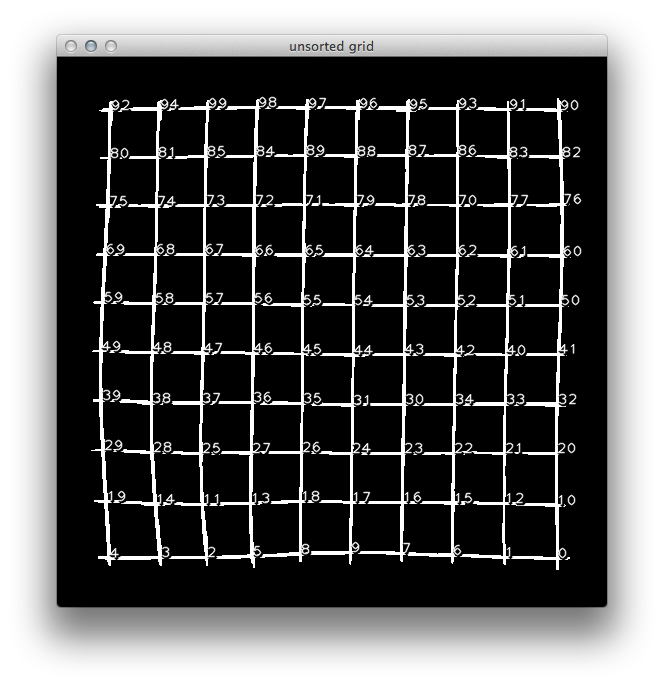
\includegraphics[width=0.49\textwidth]{Abbildungen/unsorted_grid}}
    \subfigure[sortiert]{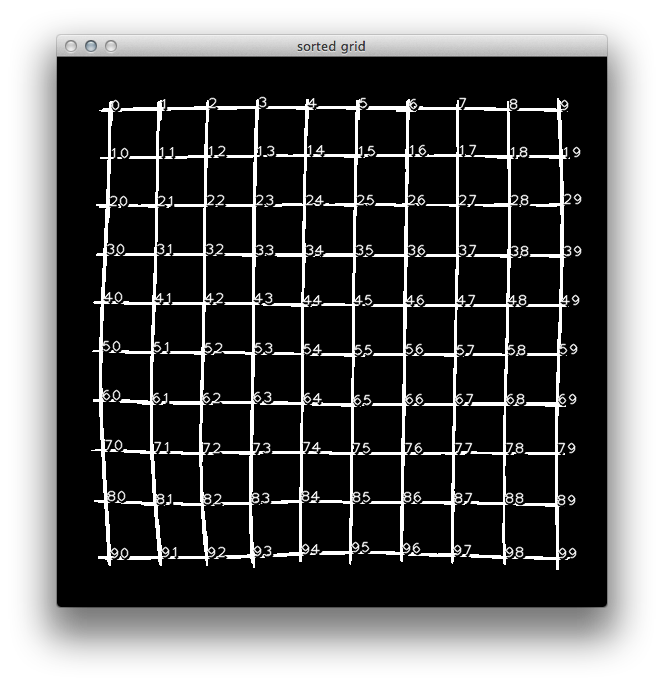
\includegraphics[width=0.49\textwidth]{Abbildungen/sorted_grid}}\hfill
    \caption{Reihenfolge der Kreuzungspunktkoordinaten}
\end{figure}


\subsection{Ziffererkennung}
Für die Ziffererkennung werden zunächst Einzelbilder der Zellen benötigt.

Die Kreuzungspunkte liegen in diesem Schritt bereits sortiert vor.
Als Referenzkoordinate für jede Zelle wird jeweils der obere linke Eckpunkt betrachtet.
Alle Eckpunkte auf dem äußeren rechten Rand des Gitters werden übersprungen.
Ist der obere, linke Eckpunkt einer Zelle gegeben, liegt der rechte obere Eckpunkt eine Position, der untere linke zehn und der untere rechte elf Positionen weiter in der Liste der Kreuzungspunkte.

Sobald die Eckpunkte einer Zelle bekannt sind, werden diese perspektivisch zu einem Quadrat transformiert, wobei die fehlerbehafteten Randbereiche abgeschnitten werden.

\begin{figure}[H]
    \begin{center}
        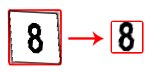
\includegraphics{Abbildungen/Ziffer}
    \end{center}
\end{figure}

\begin{lstlisting}
def solve_sudoku_ocr(src, crossing_points):
    """
    Split the rectified sudoku image into smaller pictures of letters only.
    Then perform ocr on the letter images, create and solve the sudoku using
    the Sudoku class.
    """
    numbers = []
    # enumerate all the crossing points except the ones on the far right border
    # to get the single cells
    for i, pos in enumerate([pos for pos in range(90) if (pos + 1) % 10 != 0]):

        # warp the perspective of the cell to match a square.
        # the target image "transformed" is slightly smaller than "square" to
        # cut off noise on the borders
        square = np.float32([[-10, -10], [40, -10], [-10, 40], [40, 40]])
        # get the corner points for the cell i
        quad = np.float32([crossing_points[pos],
                           crossing_points[pos + 1],
                           crossing_points[pos + 10],
                           crossing_points[pos + 11]])

        matrix = cv2.getPerspectiveTransform(quad, square)
        transformed = cv2.warpPerspective(src, matrix, (30, 30))
\end{lstlisting}

Die so isolierten Ziffern werden der OCR-Library Tesseract übergeben.
Diese wird so initialisiert, dass sie ein einzelnes Zeichen erwartet. Außerdem wurde die Liste der zulässigen Buchstaben so modifiziert, dass nur Ziffern von 0-9 erkannt werden können.
Die Library liefert einen String mit dem Ergebnis der Konvertierung zurück.

Um die Fehlerrate zu minimieren, wird das Ergebnis anschließend auf Sinnhaftigkeit überprüft.
Dazu wird zunächst versucht, das Ergebnis in einen Integer zwischen 0 und 9 zu konvertieren.

Schlägt dies fehl, kann es sich um eine Leerzelle handeln.
Wird dennoch eine Kontur mit einer gewissen Mindestgröße gefunden, wird davon ausgegangen, dass eine Zahl vorhanden ist, aber nicht richtig erkannt wird.
In diesem Fall wird der Vorgang abgebrochen und auf den nächsten Frame gewartet.

\begin{lstlisting}
    #
    # Number conversion
    #
    try:
        # strip the text from whitespace and try to convert it to an
        # integer
        n = int(ocr_text.strip())
        if not 0 < n < 10:
            return
        else:
            numbers.append(int(ocr_text.strip()))
    except:
        # skip the frame if ocr returned no number but we found a contour
        contours, _ = cv2.findContours(cv2.bitwise_not(transformed),
                                       cv2.RETR_TREE,
                                       cv2.CHAIN_APPROX_SIMPLE)
        for cnt in contours:
            area = cv2.contourArea(cnt)
            if area > 100:
                return

        # if no number or contour has been found the cell must be empty
        numbers.append(0)
\end{lstlisting}

Die erkannten Ziffern werden anschließend in das Ausgangsbild hineingeschrieben.

\begin{figure}[H]
    \begin{center}
        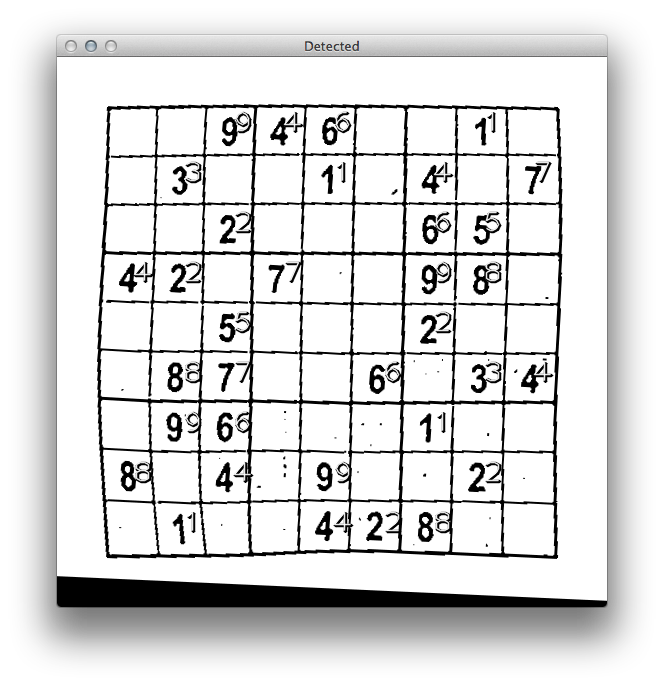
\includegraphics[width=.5\textwidth]{Abbildungen/detected}
    \end{center}
\end{figure}


\subsection{Lösung des Sudokus}
Zur Lösung der Sudokus wird die Klasse \lstinline{Sudoku} implementiert.
Ihr Konstruktor erwartet eine eindimensionale Liste aller vorgegebenen Ziffern.
Ist eine Zelle leer, so steht an dessen Stelle eine $0$.

Die Klasse enthält Methoden zum einfachen Zugriff auf einzelne Reihen, Spalten und Blöcke. Hinzu kommt eine Funktion zur formatierten Ausgabe auf der Konsole.

Zur Lösung des Sudokus wird die Library \emph{python-constraint}\footnote{http://labix.org/python-constraint} genutzt. Hiermit kann mit dem Prädikat \lstinline{AllDifferentConstraint} die Bedingung hinterlegt werden, dass in jeder Spalte und Zeile sowie in jedem Block keine Zahl doppelt vorkommen darf. Der Wertebereich der Lösungsvariablen wird auf $0-9$ eingeschränkt, bzw. bei vorgegebenen Zellen auf die gegebene Lösung.
Anschließend kann das Constraint-Problem mit einem Backtracking-Solver gelöst werden.

Die gefundene Lösung wird darauf in ein Bild gezeichnet und angezeigt.
Dabei signalisieren schwarze Ziffern bereits vorgegebene Zellen; grüne Ziffern sind Teil der Lösung.

\begin{figure}[H]
    \begin{center}
        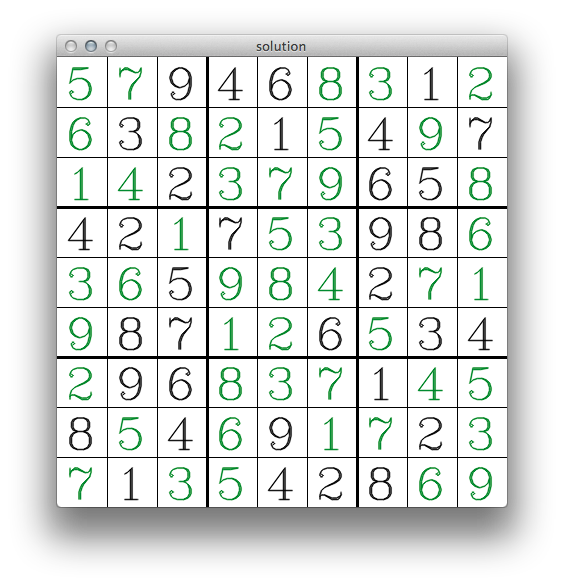
\includegraphics[width=.5\textwidth]{Abbildungen/solution}
    \end{center}
    \caption{Die generierte Ausgabe}
\end{figure}
